\documentclass[11pt]{article}
\usepackage{graphicx}
\usepackage{hyperref}
\usepackage{natbib}
\usepackage{amsmath}
\usepackage{enumitem}
\usepackage{mathtools}

\setlength{\textwidth}{6.5in}
\setlength{\headheight}{0in}
\setlength{\textheight}{8.0in}
\setlength{\hoffset}{0in}
\setlength{\voffset}{0in}
\setlength{\oddsidemargin}{0in}
\setlength{\evensidemargin}{0in}

\title{PS9}
  
\author{Shihong Pan\\ \url{https://github.com/PSH-hub24/phys-ga2000}}


\begin{document}

\maketitle

\section*{Q1}
\begin{enumerate}[label=\alph*)]
    \item We have
    \begin{equation}
        \frac{dx}{dt}=v,\quad \frac{dv}{dt}=-\omega^2x
        \label{eq:1stOrder}
    \end{equation}
    Fig \ref{fig:Q1a} plots the value of $x$ as a function of time, using the given parameters and initial conditions.
    \item Fig \ref{fig:Q1b} plots the oscillations for the initial condition $x=2$.
    \item Fig \ref{fig:Q1c} plots the oscillations for the anharmonic oscillator with $x=1$ and $x=2$. Indeed, the frequency of oscillation for $x=2$ is twice of that for $x=1$.
    \item I modified the codes and used Fig \ref{fig:Q1d} as an example of the output.
    \item Fig \ref{fig:Q1e} plots the phase space plot of the van der Pol oscillator with $\mu=1,2,4$.
\end{enumerate}

\section*{Q2}
\begin{enumerate}[label=\alph*)]
    \item Let $\theta$ be the angle between the direction of movement and the level ground. The net forces in $x$ and $y$ directions are
    \begin{align}
        F_x&=m\frac{d^2x}{dt^2}=-\frac{1}{2}\pi R^2\rho Cv^2\cos{\theta}
        \label{eq:NetForcesX}\\
        F_x&=m\frac{d^2y}{dt^2}=-mg-\frac{1}{2}\pi R^2\rho Cv^2\sin{\theta}.
        \label{eq:NetForcesY}
    \end{align}
    Note that
    \begin{align}
        v=\sqrt{(\frac{dx}{dt})^2+(\frac{dy}{dt})^2},\quad \cos{\theta}=\frac{dx}{dt}\frac{1}{v},\quad \sin{\theta}=\frac{dy}{dt}\frac{1}{v}.
        \label{eq:Subs}
    \end{align}
    Substituting eq. \ref{eq:Subs} into eq. \ref{eq:NetForcesX} and \ref{eq:NetForcesY} gives
    \begin{align}
        \frac{d^2x}{dt^2}&=-\frac{\pi R^2\rho C}{2m}\frac{dx}{dt}\sqrt{(\frac{dx}{dt})^2+(\frac{dy}{dt})^2}
        \label{eq:AccX}\\
        \frac{d^2y}{dt^2}&=-g-\frac{\pi R^2\rho C}{2m}\frac{dy}{dt}\sqrt{(\frac{dx}{dt})^2+(\frac{dy}{dt})^2}.
        \label{eq:AccY}
    \end{align}
    To obtain a unitless set of equations, define $T^2\coloneqq R/g$ and consider the following parameters:
    \begin{align}
        t'\coloneqq\frac{t}{T},\quad x'\coloneqq\frac{x}{R},\quad y'\coloneqq\frac{y}{R}.
        \label{eq:Rescale}
    \end{align}
    Substituting eq. \ref{eq:Rescale} into eq. \ref{eq:AccX} and \ref{eq:AccY} gives
    \begin{align}
        \frac{d^2x'}{dt'^2}&=-\frac{\pi}{2}A\frac{dx'}{dt'}\sqrt{(\frac{dx'}{dt'})^2+(\frac{dy'}{dt'})^2}
        \label{eq:NewAccX}\\
        \frac{d^2y'}{dt'^2}&=-1-\frac{\pi}{2}A\frac{dy'}{dt'}\sqrt{(\frac{dx'}{dt'})^2+(\frac{dy'}{dt'})^2}
        \label{eq:NewAccY}
    \end{align}
    where $A\coloneqq R^2\rho CgT^2/m$. Eq. \ref{eq:NewAccX} and \ref{eq:NewAccY} are used in the following parts.
    \item To obtain four first-order equations, the same trick as eq. \ref{eq:1stOrder} is applied, except now there are two directions $dx/dt=v_x$ and $dy/dt=v_y$. Fig \ref{fig:Q2b} plots the trajectory of cannonball in the original coordinates $x,y$ (the program gives unitless solutions, and I multiply them by $R$ to get the $x,y$ solutions). The plot assumes that the cannonball hits the level ground at the end.
    \item Fig \ref{fig:Q2c} plots the trajectories of the cannonball with $m=1, 5, 10, 15$kg. It shows that as mass increases, the cannonball goes higher in $y$ and travels further in $x$, which makes sense since the initial velocity is fixed and the de-accelerations in both directions are weaker as $m$ increases. But note that the differences between the trajectories become smaller as $m$ gets larger.
\end{enumerate}

\begin{figure}[b!]
\centering
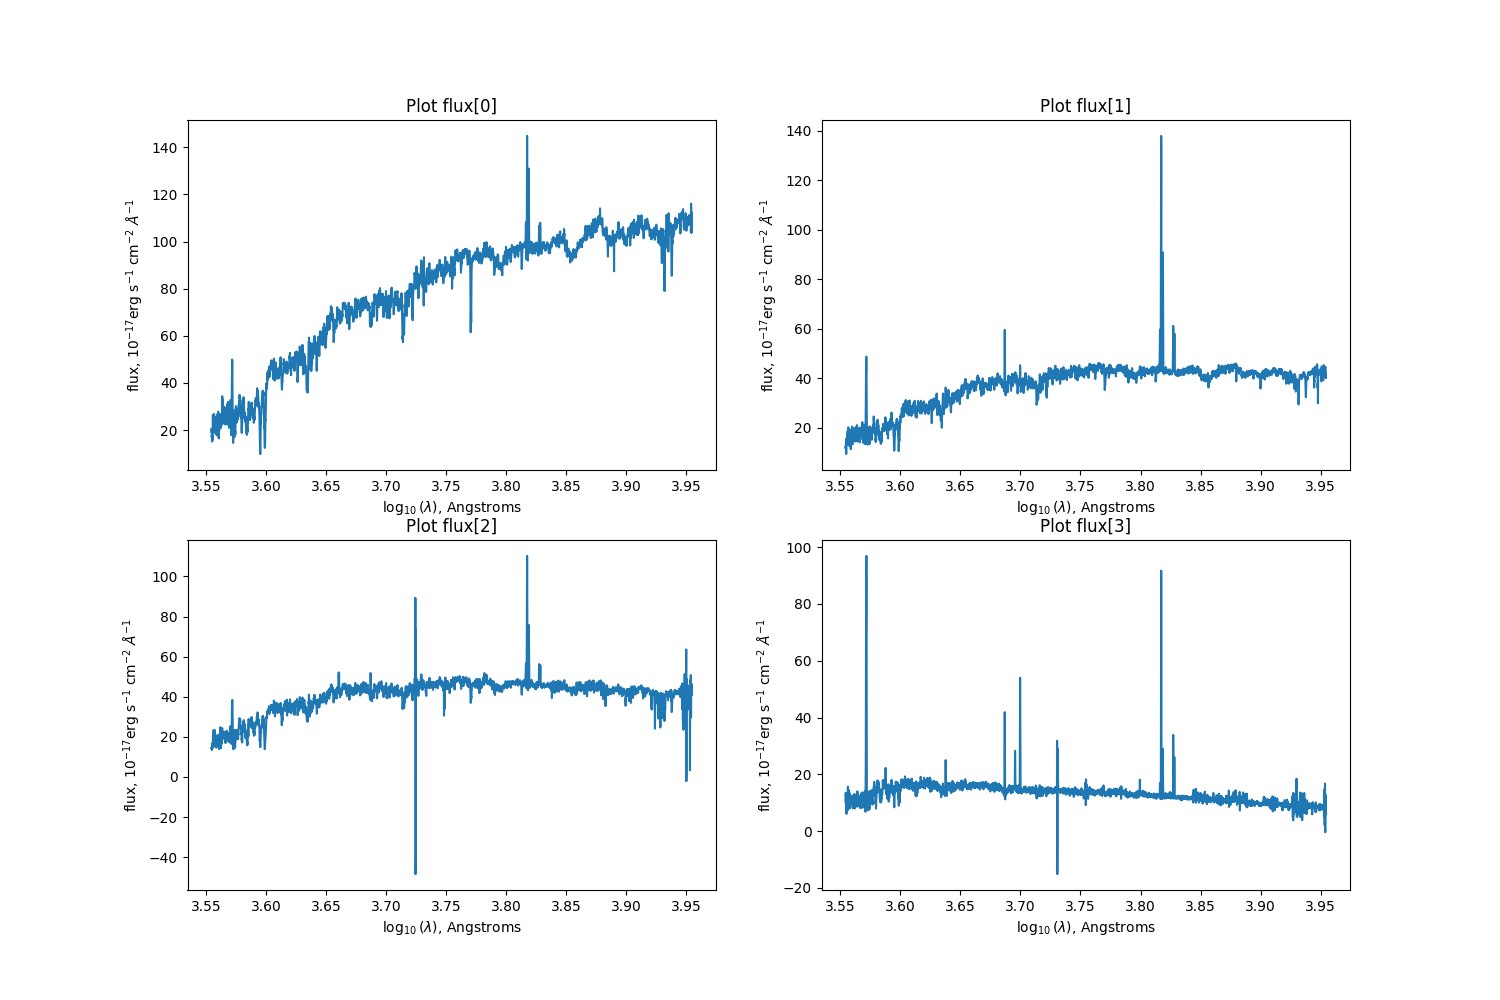
\includegraphics[width=1\textwidth]{Computational Physics/ps9Figures/q1a.PNG}
\caption{The value of $x$ of SHO as a function of time.}
  \label{fig:Q1a}
\end{figure}

\begin{figure}[b!]
\centering
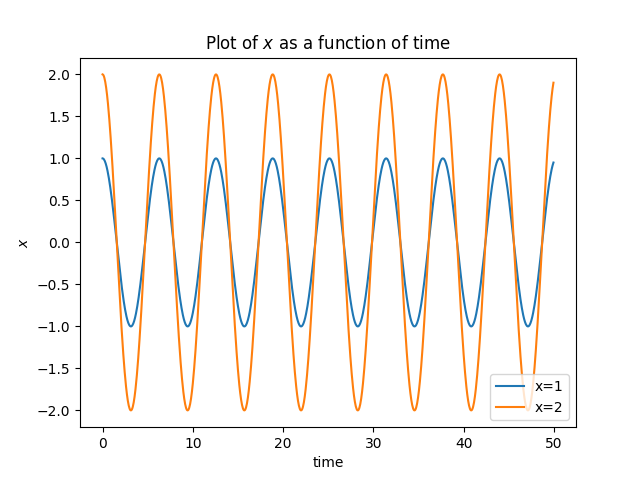
\includegraphics[width=1\textwidth]{Computational Physics/ps9Figures/q1b.PNG}
\caption{The amplitude is doubled ($x=2$).}
  \label{fig:Q1b}
\end{figure}

\begin{figure}[b!]
\centering
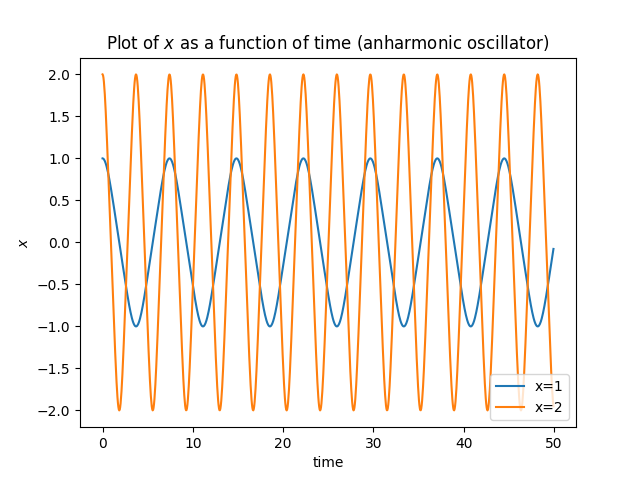
\includegraphics[width=1\textwidth]{Computational Physics/ps9Figures/q1c.png}
\caption{Anharmonic oscillator with different amplitudes.}
  \label{fig:Q1c}
\end{figure}

\begin{figure}[b!]
\centering
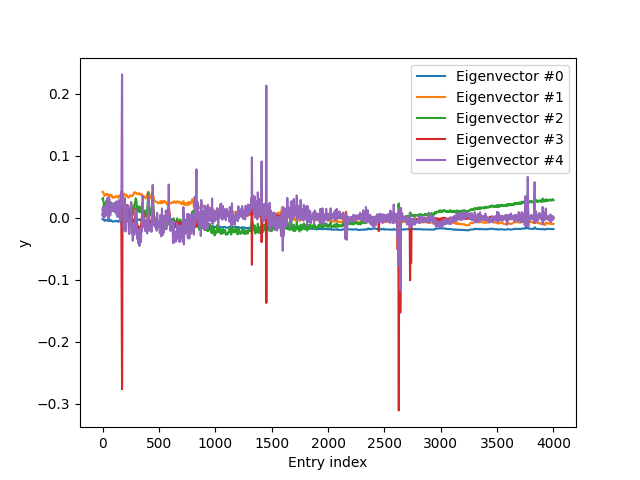
\includegraphics[width=1\textwidth]{Computational Physics/ps9Figures/q1d.png}
\caption{Example of phase space plot.}
  \label{fig:Q1d}
\end{figure}

\begin{figure}[b!]
\centering
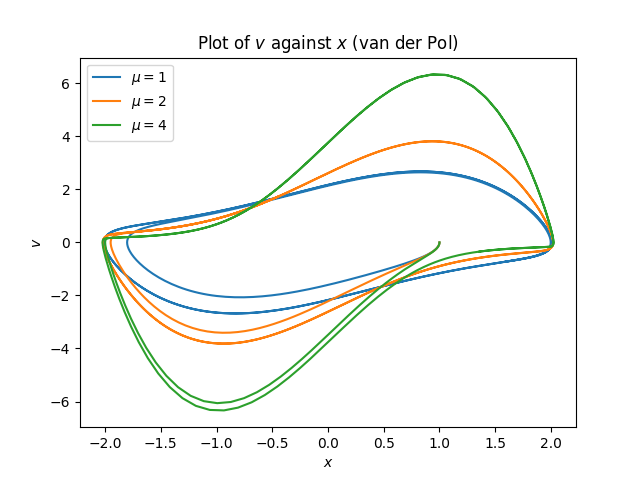
\includegraphics[width=1\textwidth]{Computational Physics/ps9Figures/q1e.png}
\caption{Phase space plot of the van der Pol oscillator with different values of $\mu$.}
  \label{fig:Q1e}
\end{figure}

\begin{figure}[b!]
\centering
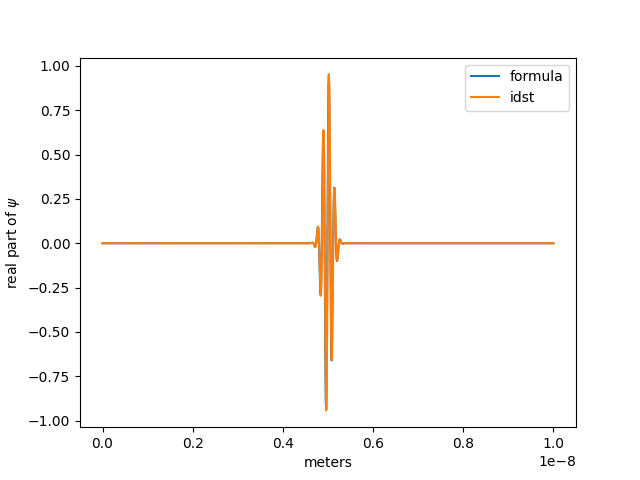
\includegraphics[width=1\textwidth]{Computational Physics/ps9Figures/q2b.png}
\caption{Trajectory of the cannonball.}
  \label{fig:Q2b}
\end{figure}

\begin{figure}[b!]
\centering
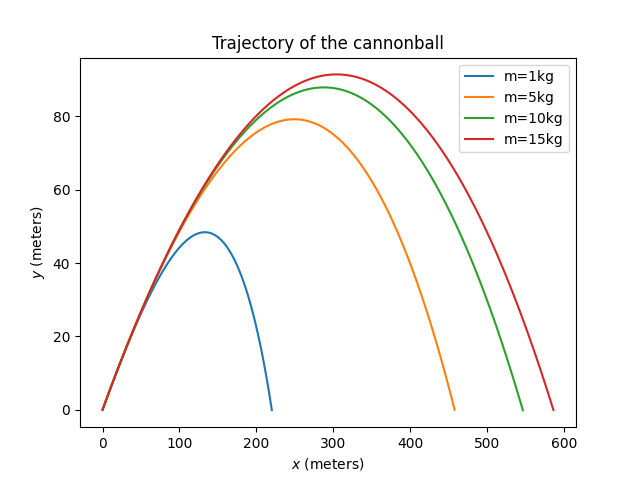
\includegraphics[width=1\textwidth]{Computational Physics/ps9Figures/q2c.png}
\caption{Trajectories of the cannonball with different masses.}
  \label{fig:Q2c}
\end{figure}



\bibliographystyle{apj}
\bibliography{example}

\end{document}

 
 
